% ~ 3-4 pages
\chapter{Reconstruction, Energy Calibration and
  Identification of Hadronic Tau Lepton Decays}
\label{sec:reconstruction}

% TauBuilder config:
% https://gitlab.cern.ch/atlas/athena/blob/master/Reconstruction/tauRec/python/TauRecBuilder.py
%
% AlgHolders:
% https://gitlab.cern.ch/atlas/athena/blob/master/Reconstruction/tauRec/python/TauAlgorithmsHolder.py
%
This chapter describes the offline reconstruction of hadronic tau decays used in
the ATLAS experiment. It summarises the reconstruction as given in Refs.\
\cite{atlas:taurec:run1, atlas:taurec:run2}, while also including recent changes
to the reconstruction algorithms. The recent changes are compiled from
documentation available in the tau reconstruction packages of the ATLAS software
framework~\textsc{Athena}~\cite{athena}. The introduction of a track selection
and classification using multivariate methods in Ref.\ \cite{duschinger} has the
largest impact on the work presented in this thesis.

% JetSeedBuilder:
% https://gitlab.cern.ch/atlas/athena/blob/master/Reconstruction/tauRecTools/src/JetSeedBuilder.cxx
Candidates for hadronic tau decays are seeded by jets formed by the
anti-$k_\mathrm{t}$ jet algorithm using a distance parameter of $R = 0.4$ on
three-dimensional clusters of calorimeter cells called \emph{TopoClusters}. The
clusters are calibrated using the local hadronic calibration (LC) to account for
the non-compensating nature of the calorimeter, dead material and out-of-cluster
energy~\cite{local_hadronic_calib}. To seed a tau candidate the jet has to
satisfy~$p_\text{T} > \SI{10}{\GeV}$ and is required to fall into the acceptance
range of the tracking system~$|\eta| < \num{2.5}$.
% At this step tau $p_\mathrm{T}, \eta, \varphi, m$ ($m$: invariant mass) are
% set to the ones of the jet seed -- what does this mean? Read up on jet algs

\section{Vertex Association}
\label{sec:reco_vertex_assoc}
% TauVertexFinder:
% https://gitlab.cern.ch/atlas/athena/blob/master/Reconstruction/tauRecTools/src/TauVertexFinder.cxx
%
% Vertex association: Tracks matched unambiguously to jets via ghost-matching by
% adding all tracks into constituent list for the jet algorithm but setting
% their energy infinitesimally small (such that the result of the jet algorithm
% is not affected due to IR-safety) and rerunning the algorithm.
% \url{https://twiki.cern.ch/twiki/bin/view/AtlasProtected/JetGhostMatching}
%
% Tracking CP recommendations
% \url{https://twiki.cern.ch/twiki/bin/view/AtlasProtected/TrackingCPPreRecsSummer2017#Track_to_Vertex_Association}
In events with multiple primary vertices the tau production vertex has to be
identified. For this reconstructed tracks that are associated to the calorimeter
jet
% via ghost-matching\footnote{Tracks matched unambiguously to calorimeter jets
% by adding the tracks with infinitesimal energy to the constituent list
% and rerunning the jet algorithm.}
and lie in a cone of $\Delta R < 0.2$ with respect to the jet axis are selected.
Tracks that fulfil $p_\text{T} > \SI{1}{\GeV}$ and basic track quality
criteria\footnote{Number of pixel hits~$N_\text{Pixel} \geq 2$, number of
  silicon hits~$N_\text{Si} = N_\text{Pixel} + N_\text{SCT} \geq 7$. Dead
  sensors on the trajectory are also counted.} are used for vertex association.
The primary vertex maximising the so called \emph{Jet Vertex Fraction} (JVF)
\begin{align*}
  \text{JVF} = \frac{p_\text{T}\text{-sum of selected tracks assigned to the vertex}}{p_\text{T}\text{-sum of selected tracks}}
\end{align*}
% \begin{align*}
%   \mathrm{JVF} = \frac{\sum_\text{Vtx.\ \& TJVA} p_\mathrm{T}}
%                                            {\sum_\text{TJVA} p_\mathrm{T}}
% \end{align*}
is associated to the tau candidate.
% \footnote{Impact parameter based association with the
%   primary vertex. $|d_0| < \SI{2.5}{mm}$ with respect to beamline and
%   $|(\Delta z_0) \sin\theta| < \SI{3}{mm}$. $\Delta z_0$ is the longitudinal
%   distance of vertex and track}

% TauAxisSetter:
% https://gitlab.cern.ch/atlas/athena/blob/master/Reconstruction/tauRecTools/src/TauAxisSetter.cxx
After the primary vertex is found, the visible four-momentum of the tau
candidate is calculated.
% Assuming constituents have zero mass.
For this the barycentre of cluster energy (LC scale) in the jet is determined.
The four-momentum of each jet constituent in the coordinate system of the
associated vertex, falling within a cone of~$\Delta R < 0.2$ with respect to the
barycentre, is summed. This defines the visible tau momentum at LC scale and the
tau-axis. The visible tau momentum at LC scale is used as a baseline for further
energy calibrations.

\section{Track Selection and Classification}
\label{sec:reco_track_sel_classif}
% TauTrackFinder:
% https://gitlab.cern.ch/atlas/athena/blob/master/Reconstruction/tauRecTools/src/TauTrackFinder.cxx
%
% TauTrackClassifier:
% https://gitlab.cern.ch/atlas/athena/blob/master/Reconstruction/tauRecTools/Root/TauTrackClassifier.cxx
Tracks reconstructed in the inner detector are associated with a tau candidate
if they are within a cone of size~$\Delta R < 0.4$ with respect to the tau-axis.
% The tracks are classified into core, wide, and other tracks: If the tracks
% fail track selection (pt > 1GeV, IPd0Max = 1mm, IPz0Max = 1.5mm, nHitPix >= 2,
% nHitSi >= 7) they are classified as 'other'.
%
% If the tracks are within the 0.2 cone they are called 'core' tracks otherwise
% if they fall into the 0.2 - 0.4 annulus they are classified as 'wide'.
%
% Loose track selection for charged pions according to TrackingCP:
% pt > 400 MeV (This cut is already applied at track reco)
% |eta| < 2.5
% NSi >= 7
% N^sh_mod <= 1 (Number of shared models = N^sh_Pix + N^sh_SCT / 2)
% N^hole_Si <= 2
% N^hole_Pix <= 1
%
% Dirk's talk in TauCP:
% https://indico.cern.ch/event/615208/contributions/2481630/attachments/1415563/2167141/TauCP_TrackClassificationTaskforce_20170220.pdf
For each track a multi-class classification is performed categorising them into
one of four track-categories: \emph{charged}, \emph{conversion},
\emph{isolation} and \emph{fake}. Tracks classified as \emph{charged} are tracks
originating from charged pions of the tau decay. \emph{Conversion} tracks are
created by long-lived secondary particles from converted photons or hadronic
interactions. \emph{Isolation} tracks are from primary particles not originating
from the tau decay and \emph{fake} tracks from combinations of unrelated space
points in the inner detector.

The multi-class classification is performed by using three boosted decision
trees~(BDT) organised into two layers. In the first layer a single BDT performs
binary classification of tracks into one of two preliminary categories:
charged/conversion and isolation/fake. The second layer uses two BDTs to
separate the preliminary categories into the four final track-categories. The
BDTs employ information on track momentum, impact parameters, number of hits in
the ID, high-threshold hits in the TRT, etc.

The track classification is used to reconstruct the charge of the tau by summing
the charge of all \emph{charged} tracks. The number of \emph{charged} tracks
also defines whether the reconstructed tau is a 1- or 3-prong decay. This
algorithm is optimised to reconstruct taus with the correct number of
\emph{charged} tracks, such that the reconstruction efficiency is maximised.
Therefore a derived track-category is used to calculate isolation variables for
the purpose of tau-identification. The \emph{modified isolation} category
consists of not classified as \emph{charged} and passing track selection
criteria:
\begin{align*}
  &p_\text{T} > \SI{1}{\GeV} & &d_0^\text{IP} < \SI{1}{mm} & &|z_0^\text{IP} \sin\theta| < \SI{1.5}{mm} \\
  &N_\text{Pixel} \geq 2 & &N_\text{Si} \geq 7 \eqcomma
\end{align*}
where $d_0^\text{IP}$ ($z_0^\text{IP}$) \todo{Check if IP is correct} is the
transverse (longitudinal) impact parameter with respect to the interaction point
and $N_\text{Pixel}$ ($N_\text{Si}$) the number of pixel (silicon) hits
including dead sensors on the trajectory. Tracks in the \emph{modified
  isolation} category are used to calculate discriminants, e.g.\ the momentum
fraction of isolation tracks, for tau-identification.

\begin{figure}[htb]
  \centering
  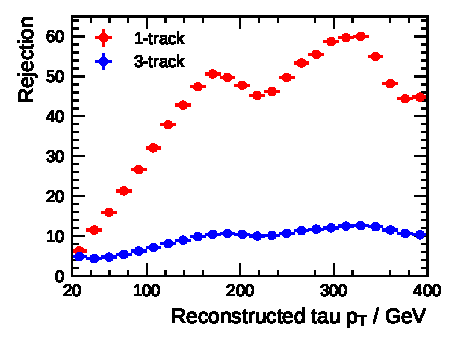
\includegraphics{./figures/bdt_perf/mva_tracking_rejection.pdf}
  \caption{Rejection due to MVA tracking. Rejection of tau candidates from
    dijets after baseline tau selection.}
  \label{fig:mva_tracking_rejection}
  \todo[inline]{Ticks are fucked. Increasing rejection with pt \textrightarrow
    increasing multiplicity of jets with higher pt. Might be a problem with
    weighting scheme?}
\end{figure}

\todo[inline]{Continue}

\todo{NTrack requirement for analyses and rejection due to this requirement}
% Tau Tracks: tracks from the direct tau decay (pions)
%
% Conversion Tracks: tracks from conversions, hadronic interactions, 'long'
% living particles MVA Tracking input (barcode > 200k -- secondary particles)
%
% Isolation Tracks: mainly tracks from the underlying event (barcode < 10k but
% not tau tracks)
%
% Fake Tracks: not truth matched (10k < barcode < 200k) (includes pilup?)
%
% barcode < 200k -- primary particles
%
% variables: jetseed pt, track eta, z0SinThetaTJVA, rConvII, dRJetSeedAxis, d0,
% qOverP, nInnermostPixelHits, nPixelSharedHits, nSCTSharedHits, eProbabilityHT,
% nPixHits, nSiHits
% Impact params: reject conversion (d0), isolation and fake tracks (z0)
% Pixel, Si-Hits: rejection against conversions (missing hits)
% shared hits: intent is to recover merged tracks
% eProbabilityHT: Conversion tracks
% qOverP, dR: IT, FT

\section{Energy Calibration}
\label{sec:reco_energy_calib}
% TauCalibrateLC:
% https://gitlab.cern.ch/atlas/athena/blob/master/Reconstruction/tauRecTools/Root/TauCalibrateLC.cxx
%
% 5 eta bins: [0.0, 0.3, 0.8, 1.3, 1.6, 2.4]
% pile-up slopes for 1P and 3P for each eta bin
% mean pile-up for 1P and 3P
% A calibration function for 1P and 3P for each bin
%
% Offset calculated as
% offset = slope * (reco. num of PU vertices - average number of PU vertices)
% energyLC = ptDetectorAxis()
% if energyLC - offset <= 0: set offset to 0
% energyPUCorr = energyLC - offset
% calibConst = func(nProng, eta; energyPUCorr)
% if calibConst <= 0: calibConst = 1.0
% energyFinal = energyPUCorr / calibConst
%
The visible momentum measurement of the hadronic tau decay at LC scale is not
optimised to accuratly reflect the true visible momentum. Additional corrections
for energy contributions due to pile-up and energy depositions outside of the
$\Delta R < 0.2$ cone need to be taken into account. Therefore, an energy
calibration is applied to the reconstructed object accounting for pile-up and
the detector response in different $\eta$ regions.

\todo[inline]{Continue}

\todo{Motivation: LC scale not optimised for tau energy measurement; e.g.
  hadronic composition of the final state, pile-up, cone size of 0.2. Reduce
  bias and improve resolution} To get the visible tau energy a further energy
calibration is applied to the tau candidates to account for pileup and the
detector response in different $\eta$ regions. First the pileup contribution
$E_\text{PU}$ to the energy at LC-scale $E_\text{LC}$ is estimated using
\todo{Does the LC-scale already account for the average pile-up? Otherwise the
  parametrisation subtracting the average number of pile-up vertices would not
  make sense! The LAr bipolar calorimeter signal should cancel the in-time
  pile-up with the out-of-time pile-up.}
\begin{align*}
  E_\text{PU} &= m\left(|\eta|\right) \times \left( N_\text{Vtx.}^\text{PU}
                - \langle N_\text{Vtx.}^\text{PU} \rangle \right) \eqcomma
\end{align*}
where $m$ is the average pile-up contribution to the energy at LC-scale (is a
function of $|\eta|$) parametrised in bins of eta separately for 1- and
multi-prong taus. Finally the energy is corrected for the detector response (in
bins of $|\eta|$ and separately for 1- and multi-prong).
\begin{align*}
  E_\text{TES} &= \frac{E_\text{LC} - E_\text{PU}}
                 {\mathcal{R}(|\eta|, E_\text{LC} - E_\text{PU})}
\end{align*}
The detector response function $\mathcal{R}$ is fitted to the mean of the
$\frac{E_\text{true}}{E_\text{LC} - E_\text{PU}}$ distributions (from a Gaussian
fit) in simulation for each bin using a function with an empirical form.

\section{Shot Reconstruction}
\label{sec:shot_reco}
\todo[inline]{Move this somewhere else}

\todo[inline]{Whats the purpose? Reconstruct individual photons in
  $\pi^0$-decay}

% TauShotFinder
% https://gitlab.cern.ch/atlas/athena/blob/master/Reconstruction/tauRecTools/src/TauShotFinder.cxx
Local maximum in EM1 strip layer determined by cells within 0.2 (0.4?) to the
tau axis. Cells required to have above \SI{100}{\mega\electronvolt}. Two seed
cells can't be neighbours in eta. Seed cell must be local maximum in eta (both
neighbours are required to have lower cell energy). Shot construction: Seed
cells neighbouring a seed cell in phi direction are merged (only the highest pt
neighbour is merged). A cluster is built in a 5 (eta) x 1 (phi) window around
the seed or 5 x 2 in case a neighbouring seed was merged in. The four-momentum
is set to the cell energy/eta/phi of the seed cell or in case of merged seeds to
the sum of the seed cell pt and the barycentre of energy in phi direction. The
number of photons in the shot is calculated as a function of 5 $|\eta|$ bins
($0, 0.8, 1.39, 1.51, 1.8, \infty$). If the seed energy (energy in a window of
width 3x1(2)) is smaller then a threshold no photon is counted. If it exceeds
the threshold \{430 MeV, 300 MeV, crack, 330 Mev, 350 MeV\} one photon is
counted. In case the shot energy exceeds 10 GeV the photon is counted twice.


\todo{Cite ATHENA?}
\cite{atlas:taurec:run1}
\cite{atlas:taurec:run2}
\cite{atlas:taurec:decaymodes}

%%% Local Variables:
%%% mode: latex
%%% TeX-master: "mythesis"
%%% End:
